\documentclass[UTF8]{ctexart}

\usepackage{amsfonts} % 数学字体支持
\usepackage{amsmath} % 数学啊啊支持
\usepackage{makeidx} % 索引工具
\usepackage{graphicx} % 图片支持
\usepackage{booktabs} % 三线表支持
\usepackage{appendix} % 附录支持
\usepackage{fancyvrb} % 代码支持
% 页面设定
\usepackage[left=1.25in,right=1.25in,top=1in,bottom=1in]{geometry}
% 图标设定
\graphicspath{{figure/}} % 设定图表所在文件夹
% 附录设定
% \renewcommand{\appendixtocname}{附录} % 设定附录目录标题
\renewcommand{\appendixname}{附录} % 设定附录标题,好像没用
\renewcommand{\appendixpagename}{附录} % 设定附录大标题
% 参考文献设定
\makeindex
\bibliographystyle{unsrt} % 按照引用顺序排序

\title{工业数据统计分析与应用课程报告\\——用于线性回归的面部识别算法}
\author{刘永峰}
\date{\today}

\begin{document}
\maketitle % 标题页
\begin{abstract}
    本文旨在对用于面部识别的线性回归分类算法(Linear Regression Classification)进行重现并呈现实验结果。该线性回归分类算法将待识别图像表示为根据类进行划分的一组图像的线性组合,它使用最小二乘法对前述问题的系数向量进行求解并生成预测器,并根据不同类预测器生成的预测结果与待识别图片的距离来判断其所属类别。本文将该算法用于AT\&T面部图像数据库并进行了有关参数的调试。另外还对跟随LRC算法同时提出的用于处理人脸图像中连续覆盖物的模块化LRC(Modular LRC)进行了描述,但由于时间原因,并未进行重现。\\
    \textbf{关键词}:面部识别,连续遮挡,线性回归算法
\end{abstract}
\section{研究背景与意义}\label{sec-1}
面部识别技术是目前人工智能与机器视觉研究领域的重点技术之一,有着广阔的应用前景,如摄像头监控、刷脸支付及身份识别等。
面部识别算法的效果依赖于多种有关工具的设计和选择。首先,一个\(a \times b\)维的灰度面部图像可以被表示为在原始图像空间(image space)的\(ab\)维的向量。但是如果直接处理类似数据量的原始数据会导致严重的维数灾难,以至于在一些情况下完全无法完成处理。所以研究者希望在特征提取阶段将原始数据在保证能够对面部进行区分的条件下降维到面部空间(face space)。在这种目标的驱动下产生并应用了一系列的特征提取方法,如主成分分析(Principle Component Analysis, PCA)\cite{b1}、线性判别(Linear Discriminant Analysis, LDA)\cite{598228}和独立成分分析(Independent Component Analysis, ICA)\cite{comon1994independent,bartlett2001independent}等等。前述方法大体上可以分为两种类型:重构型(reconstructive)和判别型(discriminative)。重构型方法对于受污染像素的处理更为有效,而判别型的方法则相对更为适合原始数据较为干净的情况\cite{duda2012pattern}。除了以上这些传统的方法之外,研究者发现似乎诸如下采样(downsampling)、随机投影等等一些非“正统”的方法方法在实际应用上也同样有效,即特征空间的选择看似并非是关键因素\cite{4483511}。于是,确定特征空间维度和分类器的设计就成了影响算法效果的重中之重。\par
本文基于Imran Naseem等人发表于2010年的文章Lnear Regression for Face Recognition\cite{5506092}中的LRC算法进行重现。在该文中,作者提出了简单有效LRC算法用于进行面部识别。该算法基于这样一条准则,即\textit{某种类别的所有样本都会落在同一个线性子空间内}\cite{598228,1177153},从而使用线性回归对面部识别问题进行处理。其中反映待分类图像与类模型之间关系的参数向量由最小二乘估计给出。最终,根据每类对待分类模型预测的准确度来确定图像所属类别。该方法可被视作一种最近邻子空间(Nearest Subspace, NS)方法。\par
LCR算法所基于的最重要的工作在文献\cite{4483511}中进行了描述。其在训练阶段使用所有的下采样后的图像用于生成字典矩阵(dictionary matrix),然后将待分类图像表示为各个字典矩阵中向量的线性组合,从而构成了一个病态逆问题(ill-conditioned inverse problem)。该问题中所存在系数向量稀疏性问题(sparsity of the vector of coefficients)可以利用线性范数极小化(\(l_1\)-norm minimization)方法来求解。文献\cite{1114855}中,局部线性回归(Locally Linear Regression, LLR)方法被用于处理朝向不同的面部图像。该文献阐述了面部侧面图像和正面图像的近似线性映射关系并给出了将该问题的求解化为一个累进解的预测问题的方法。对于变化较为严重的摆姿,则对不同朝向的图像进行采样,得到很多交叠的局部段落,从而可以使用这些小的段落,对正面人像进行分类。LLR算法在校准较为粗略的面部图像识别之中获得了一些优异的表现。文献\cite{1114855}中提出了一种两阶段的方法,该方法在特征提取阶段将小波分解(wavelet decomposition)和判别分析(discriminant analysis)结合,提取的特征用于构建特征平面和特征空间。最终将待分类图像投影到子空间之中并根据最小距离来判断所属类别。而LCR算法则采用更为基础的方法得到了较之前两例基准算法更为优异的表现。\par
进一步的,有研究者还针对严重的连续遮挡物提出了一种图像的模块化表示方法\cite{323814},并给出了模块化的LCR算法用于求解该类图像的识别问题。该方法将存在连续遮挡的图像进行分割,并对每个分割进行判别,然后使用名为基于距离的证据融合(Distance-based Evidence Fusion, DEF)算法对最终结果进行预测。分割方式的好坏则是通过对中间决策(即不同分块的类型判别结果)构成的距离矩阵进行评估来进行判断。该类方法的优势有:第一,通过距离矩阵的评估和证据融合避免了遮挡部分参与并影响判断结果;第二,证据融合使最终判断结果优于最优的独立分块的判断结果。\par
以下内容将分为几个部分进行阐述:第二部分介绍了LRC和模块化LRC算法,第三部分将对实验结果进行大致描述,第四部分是总结与展望的内容。
\section{用于面部识别的线性回归算法}\label{sec-2}
以下内容将对面部识别的LRC算法和用于处理连续遮挡的图像的模块化处理方法分别进行阐述。
\subsection{线性回归分类器}
该方法简而言之就是使用多组分类后的含标签图像向量构成预测器,并估计每组图像向量集对目标图像向量的\textbf{线性组合},估计最为精确的那一类——即线性组合后得到的响应向量距离目标图像向量最近者即为目标图像所属的类型。具体流程如下文所述。\par
设有\(N\)个互相区别的类,其中第\(i\)类中包含\(p_i\)个训练图像,\(i=1,2,...,N\)。每个\(a \times b\)维的灰度训练图像可以被表示为\({\stackrel{(m)}{u_i}} \in {\mathbb{R}^{q \times 1}}, i = 1,2,\dots,N\)且\(m = 1,2,\dots,p_i\)。其中每个训练图像均被下采样到\(c \times d\)维,并且通过列连接(column concatenation)转换为列向量,即\({\stackrel{(m)}{u_i}} \in {\mathbb{R}^{q \times 1}} \rightarrow {\mathbf{w}_i} \in \mathbb{R}^{q \times 1}\),其中\(q=cd,cd<ab\)。每个图像向量均进行归一化令灰度最大值像素值为1。基于同一个类型的样本均落在同一个线性子空间中的准则,通过将同一类的\(q\)维图像向量进行堆积,可以得出如下的类型划分模型
\begin{equation}
    {\mathbf{X}_i = [\stackrel{(1)}{\mathbf{w}_i} \quad \stackrel{(2)}{\mathbf{w}_i} \dots \stackrel{(p_i)}{\mathbf{w}_i}] \in \mathbb{R}^{q \times p_i}},\quad i=1,2,\dots,N
\end{equation}
其中每个向量\(\mathbf{{\stackrel{(1)}{w_i}}}\)构成的子空间\(\mathbb{R}^{q}\)也是\(\mathbf{X_i}\)的列空间。即每个类型\(i\)都可以被表示为子空间\(\mathbf{X}_i\),\(\mathbf{X}_i\)也被称作类型\(i\)的回归器(regressor)或者预测器(predictor)。如果设\(z\)是一个无标签灰度图像,则我们的问题就可以表示为求\(z\)所从属的类别\(i\),此处\(i=1,2,...,N\)。我们将\(z\)也做与训练图像相同的转换,即进行归一化和列连接将之转换为图像向量\(\mathbf{y}\),即\(\mathbf{y}\in\mathbb{R}^{q \times 1}\)。如果\(\mathbf{y}\)属于第\(i\)类,则它可以表示为相同类别的训练图像的线性组合(也就是说它与该组训练图像会落在相同的子空间内),即
\begin{equation}\label{eq-2} % 注意交叉引用标签命名,不能直接使用eq2好像
    \mathbf{y}=\mathbf{X}_i\beta_i,\quad i=1,2,\ldots,N,
\end{equation}
% \eqref用于公式的交叉引用
其中\(\beta_i\in\mathbb{R}^{p_i \times 1}\)是参数向量,已知\(q \ge p_i\),公式\eqref{eq-2}中的系统是\textbf{良态}(well conditioned)的,从而可以使用最小二乘估计来估计\(\beta\),公式如下
\begin{equation}\label{eq-3}
    \hat{\beta}={(\mathbf{X}^T_i\mathbf{X}_i)^{-1}\mathbf{X}^T_i\mathbf{y}}
\end{equation}
\par
从而得到的参数向量\(\beta\)以及预测器\(\mathbf{X}_i\)可以用来预测每个类的响应向量(response vector),公式及相关变换如下
\begin{equation}\label{eq-4}
    \begin{split}
        & \hat{\mathbf{y}}_i={\mathbf{X}_i\hat{\beta}_i}\\
        & \hat{\mathbf{y}}_i={\mathbf{X}_i{(\mathbf{X}^T_i\mathbf{X}_i)}^{-1}{\mathbf{X}^T_i\mathbf{y}}}\\
        & {\hat{\mathbf{y}}_i}={\mathbf{H}_i\mathbf{y}},
    \end{split}
\end{equation}
式中预测向量(响应向量)\(\hat{\mathbf{y}}\in\mathbb{R}^{q \times 1}\)是\(\mathbf{y}\)在第\(i\)个子空间中的投影。实际上也就是说\(\hat{y}_i\)是在子空间\(i\)中相距观察向量(observation vector)\(\mathbf{y}\)欧氏距离最近的向量。而其中将\(\hat{\mathbf{y}}\)转换为\(\mathbf{y}\)的矩阵\(\mathbf{H}\)被称作帽子矩阵(hat matrix)。有了\(\hat{\mathbf{y}}_i\)和\(\mathbf{y}\),我们就可以计算\(\mathbf{y}\)和不同类的估计向量\({\hat{\mathbf{y}}}_i\)之间的欧氏距离\(d_i(\mathbf{y})\)
\begin{equation}\label{eq-5}
    d_i(\mathbf{y})={\|\mathbf{y}-{\hat{\mathbf{y}}}_i\|}_2,\quad i=1,2,\dots,N
\end{equation}
得到了两者的欧氏距离之后,其中与\(\mathbf{y}\)相距欧氏距离最小的\(\hat{\mathbf{y}}_i\)所属的类别\(i\)就是\(\mathbf{y}\)所属的类别,即
\begin{equation}
    \underbrace{\min}_i d_i(\mathbf{y}),\quad i=1,2,\dots,N.
\end{equation}

\subsection{线性回归分类器中的图像模块化方法}
\texttt{作者在文献\cite{5506092}中还提出了一种用于处理连续遮蔽的模块化LRC算法,由于使用的带有遮蔽的面部图像数据库在文中需要进行手动对齐,基于工作量和报告上交时间考虑并未进行重现,但在此也一并介绍之。}\par
局部遮挡的面部识别问题可以用图像模块化方法来处理,因为局部连续遮挡物虽然遮挡范围可能有所不同,但是由于其是连续的,所以只是污染了一部分像素,所以采取特定方法将之区分即可。而分块的图片表示方法可以有效地处理这类问题。文献\cite{5506092}中的分块处理方法则是将原始图像分为几个部分,每个部分都进行独立的线性回归,然后将所有的部分得到的证据进行融合得出最后的分类结果。当然最简单的决策融合方法可能就是多数表决(majority voting)\cite{323814}了,但该方法将污染部分和未污染部分等效看待,可能会引发问题。试想如果四块图像三块都是被污染的部分,那么如果进行多数表决那么无论无污染部分和原始图像匹配有多么显著,最终结果仍然是被污染部分的决策结果占据优势,而毫无疑问,被污染部分在决策过程中不应当拥有这样的权重。另问题更为复杂的是污染分布并不是先验的,可能分布在非面部区域,也可能分布在面部区域。据此,有人提出了复杂的污染像素剔除算法\cite{1580480}。\par
而对于这种问题,参照文献\cite{5506092}中给出的方法则较为简单。该方法基于距离分类,自然而隐式地降低了被污染子图像的决策权重,从而显著提高了分类精度。该方法被称为“基于距离的证据融合(Distance-based Evidence Fusion)”,具体方法如下:
假设每个训练图像均被划分为\(M\)个部分,每个部分用\(v_n,\ n=1,2,\dots,M\)表示。其中全部\(p_i\)个训练图像的第\(n\)个子图像均按照章节\ref{sec-2}所述进行下采样和列连接处理并最终构成分类-分区子空间\(\mathbf{U}^{n}_i\):
\begin{equation}
    \mathbf{U}^{(n)}_i=[\stackrel{(1)^{(n)}}{\mathbf{w}_i}\stackrel{(2)^{(n)}}{\mathbf{w}_i}\ldots\ldots\stackrel{(3)^{(n)}}{\mathbf{w}_i}],\quad i=1,2,\dots,N.
\end{equation}
每个分类均可以被表示为\(M\)个子空间,于是我们得到了具有\(M\times N\)个子空间的分类模型。对于待分类图像我们也划分为\(M\)块并对每块进行列连接处理转化为图片向量\(\mathbf{y}^{(n)},n=1,2,\dots,M\)。已知\(i\)为该待分类图像所属的类别,那么\(\mathbf{y}^{(n)}\)就应当位于分类器\(\mathbf{U}^{(n)}_i\)的第\(n\)个子空间,即应当满足
\begin{equation}
    \mathbf{y}^{(n)}=\mathbf{U}^{(n)}_i\beta^{(n)}_i
\end{equation}
于是乎类似于LRC的逻辑,参数向量和预测图像向量可以由下式计算得出:
\begin{align}
    \hat{\beta}^{(n)}_i&={[(\mathbf{U}^{(n)}_i)^T\mathbf{U}^{(n)}_i]}^{-1}(\mathbf{U}^{(n)}_i)^T\mathbf{y}^{(n)},\\
    \hat{\mathbf{y}}^{(n)}_i&=\mathbf{U}^{(n)}_i{\hat{\beta}}^{(n)}_i;\quad i=1,2,\dots,N.
\end{align}
\par
同时估计图像向量和原始图像向量的距离也由类似LRC的逻辑给出:
\begin{equation}
    d_i(\mathbf{y}^{(n)})=\|\mathbf{y}^{(n)}-\mathbf{y}^{(n)}_i\|_2;\quad i=1,2,\dots,N.
\end{equation}
\par
现在对于分块\(n\)我们可以进行其所属分类的决策了,该决策被称为中间决策(intermediate decision),表示为\(j^{(n)}\),该决策类似前文,由最小距离给出,而我们暂时需要的是该决策所对应的距离:
\begin{equation}
    d^{j^{(n)}}=\underbrace{\min}_i d_i(\mathbf{y}^{(n)})\quad i=1,2,\dots,N
\end{equation}
至此我们有\(M\)个子图像决策距离了,融合决策的步骤也很简单,就是直接选取这\(M\)个中间决策中距离最小的那个所对应的决策,即为最终决策:
\begin{equation}
    Decision=\arg{\underbrace{\min}_j}d^{j^{(n)}}\quad n=1,2,\dots,M.
\end{equation}
\section{实验结果}\label{sec-3}
算法重现之后对该算法进行了一些实验,实验并非如原文献中出于对比不同算法识别准确度,而是想对比了其中一些具体的设置以及使用的处理方法如重采样等所能导致的算法运行的结果差异并期望能够找到最优的方法组合。使用的测试数据为AT\&T面部图像数据库。最终结果表明对算法的重现的结果与文献中所展示结果基本没有差异,达到了重现的要求;另外进行的有关下采样方法选择、下采样后的图像空间维度等等对算法表现的影响将在下文详述。
\subsection{AT\&T面部数据库}
AT\&T面部数据库\footnote{http://www.cl.cam.ac.uk/research/dtg/attarchive/facedatabase.html}是由剑桥大学AT\&T研究室发布的一个人类面部图像数据集,该数据集包含1992年1月-1994年1月在AT\&T研究室拍摄的用于进行人脸识别实验的一组照片。该组照片包含40个不同的人每人10张不同角度与表情的图像,拍摄环境均为暗色背景(一组照片如\ref{fig-example_ATT}所示)。其照片分辨率均为92\(\times\)112。
\begin{figure}[htbp]
    \centering
    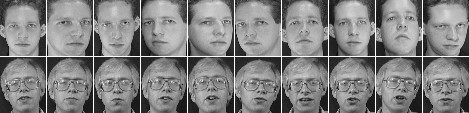
\includegraphics[scale=0.7]{ATT.jpg}
    \caption{AT\&T数据库照片示例}\label{fig-example_ATT}
\end{figure}
\subsection{实验方案}
实验按照文献\cite{1261097}所使用并推广的评价方案进行设置,即前5张图像作为训练集而后五张图像作为测试图像,文献\cite{4359331}中进行实验的另外一种“leave-one-out”的评价方案没有进行实验。\par
实验中对算法的不同环节部署了不同的设置并进行了对比,以下是进行对比的环节。
\subsubsection{标准化方法}
本实验使用的标准化方法均为min-max标准化方法,公式如下:
\begin{equation}\label{eq-14}
    a^*=\frac{x-min}{max-min}
\end{equation}
\par
在参数选择的过程中,公式\eqref{eq-14}中的\(min\)和\(max\)的值在初次进行实验时采用的是基于样本数据即根据当前图片灰度值中的最大/最小值确定的,但是在接下来的代码编写过程中意识到该方式可能有些不妥,于是考虑256位深的灰度图像的原生灰度范围对\(min\)和\(max\)进行定义,即\(min=0,max=255\)。之后进行了有关实验对比确认是否会存在差异。
\subsubsection{下采样方法}
\begin{table}[htbp]
    \centering
    \caption{不同滤波器效果比较\protect\footnotemark}\label{fig-filter_comparison}
    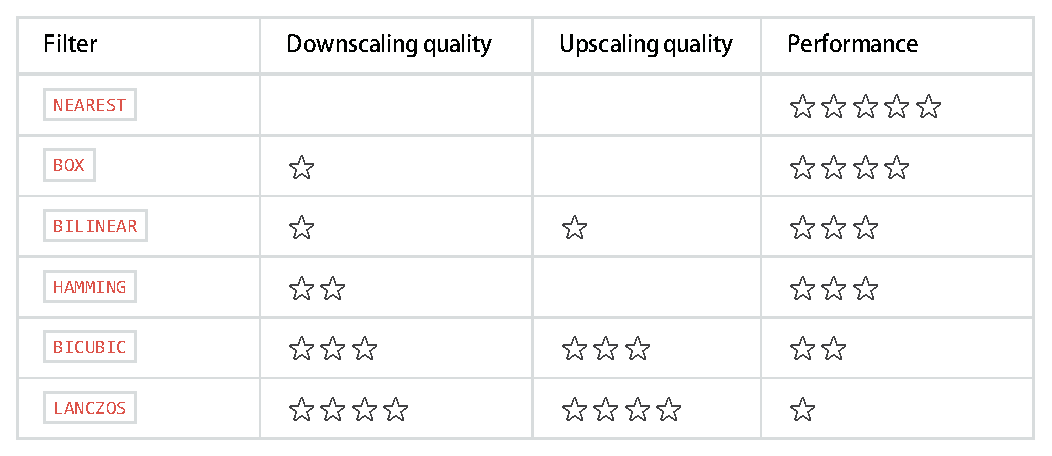
\includegraphics[scale = 0.7]{Filter.eps}
\end{table}
\protect\footnotetext{https://pillow.readthedocs.io/en/5.2.x/handbook/concepts.html\#concept-filters}
本实验中使用的下采样方法是由Pillow\footnote{http://pillow.readthedocs.io/
}——即Python PIL图像处理库的一个广泛使用的分支——提供的图像缩放滤波器(如图\ref{fig-filter_comparison}所示)中的三种:NEAREST、BOX以及LANCZOS。三种方法的原理如下:\par
NEAREST即最近点采样滤波器,它进行图像重采样的方式是选择最近的一个像素而完全不管其余的像素。\par
BOX滤波即盒式滤波,对需要保留的像素位置周围一个箱形范围内的像素进行平均,在下采样中其机制可以由下述公式简单表示:
\begin{equation}\label{eq-15}
    p_k=\left({\sum_{i\in win(k)}{I_i}}\right)/s^2
\end{equation}
式中s为缩放比例。具体关于非整数倍采样的重叠区域如何进行处理等具体细节不在此详述。\par
LANCZOS滤波则引入了正弦函数对周围像素的权重进行差异化处理用于合成目标像素,对与中心像素距离逐渐增大的像素采用逐渐减小的权重,故相比盒式滤波质量要高一些。\par
几种滤波方式的比较如图\ref{fig-filter_comparison}所示。

\subsubsection{下采样比例}
\begin{table}[htbp]
    \centering
    \caption{下采样比例设置}{原始图像feature dimension为\(92\times 112=10304\)}\label{tab-downsampling_factor}
    \begin{tabular}{ccccccccc}
        \toprule
        Downsampling Factor & 40 & 35 & 30 & 25 & 20 & 14 & 10 & 5 \\
        Feature Dimension & 6 & 9 & 12 & 16 & 30 & 56 & 99 & 396 \\
        \bottomrule
    \end{tabular}
\end{table}
下采样比例直接造成最终的训练图片和测试图片的分辨率差异,即影响留存信息的比例以及来源。如前文所述,较之于下采样方式,下采样比例也就是留存数据的维度对于图像识别精度可能更为关键。所以本次实验采用不同的下采样比例进行了多次实验。所使用的下采样变化由手动设定,旨在尽可能地反映变化趋势(如表\ref{tab-downsampling_factor}所示)。
\subsection{实验结果及分析}
\begin{figure}[htbp]
    \centering
    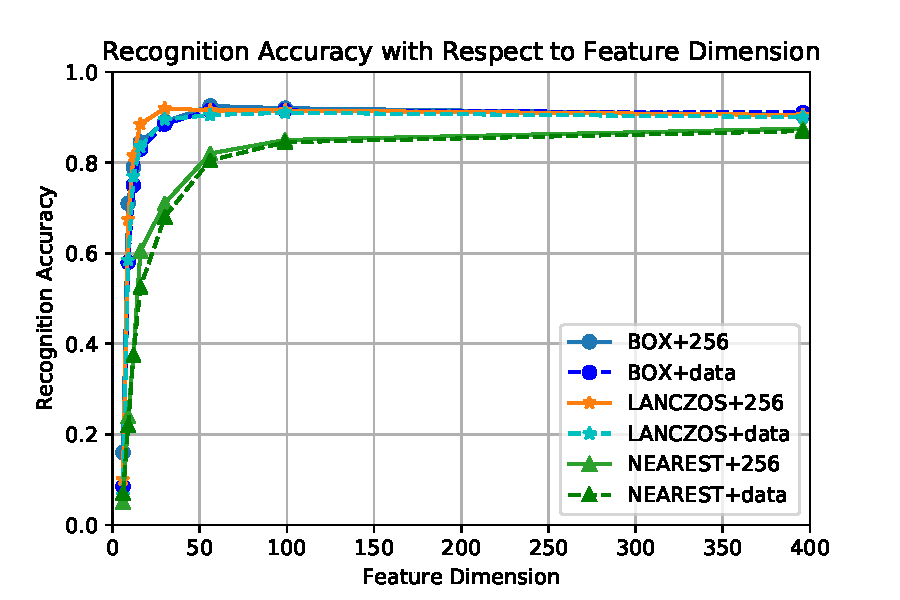
\includegraphics[scale=0.7]{RA_Method.pdf}
    \caption{不同设置下的LRC识别精度差异}{BOX、LANCZOS、NEAREST分别为不同的图像滤波器;256代表定值归一化,data代表基于样本数据的归一化}\label{fig-result_method}
\end{figure}
基于前文所述的设置差异,最终结果如图\ref{fig-result_method}所示。
由图中首先可以看出无论是采用何种设置,所有实验的识别精度基本上都随着特征维度的提升而提升,并且在一开始随着特征维度的增大精度上升较快,一旦特征维度到达50之后精度最高且之后基本保持稳定(约0.9左右),甚至可能还会随着特征维度的上升精度产生小幅下降,该特性与原始文献中的特性保持一致。该结果出乎意料地表明对于AT\&T数据库实际上低精度图片已经能够提供足够的信息用于区分不同类别即不同拍摄对象的面部,但深入思考这种结果可能并不代表这样的低精度足够区分样本数量较大的并且个体间差异较小的面部图像数据。推测可能随着样本的增大和样本间差异的减小,为了提高精度依然需要较高的特征维度;而在使用较高特征维度的情况下存在的精度下降现象推测可能是图像噪声的影响,可能是90年代相机感光元件的发展水平制约了图像的“纯粹”程度。综合以上推测,使用LRC算法划分差异较小的类型需要在保证图像质量的前提下使用较高的特征维度,该结论也与人们普遍的直观认识相符。\par
进一步地,可以看出使用NEAREST即最近点采样滤波器的实验结果最差,但是随着维度增高精度逐渐向其他方法靠拢(毕竟越来越接近原图,特征维度到原图像维度时滤波是不起作用的,结果确实应当相同),产生该结果的原因只管而言应该是最近点采样滤波在低维度时对原始信息的保留与概括程度过低,得到的数据不具有代表性。另外两种滤波方式得到的结果相当近似,说明具有平均特性的不同滤波方式对该组数据集识别的影响不大。\par
而对比不同的标准化处理方式可以看出定值(\(max=255,min=0\))标准化方式表现较样本min-max标准化方式稍显优异。可能样本数据的不稳定性产生了这样的结果。但是这样的标准化方式对于整体光照强度不同的图像的识别可能有其独特的优势。\par
对于该组数据最优秀的设定为BOX+定值标准化+56维特征维度\footnote{实际上LANCZOS+定值标准化+30特征维度得到的结果92.0\%与之相仿,而运行效率而言LANCZOS+定值标准化+30特征维度的7338.36ms优于BOX+定值标准化+56特征维度的8622.93ms运行时间。但当前主要比较识别率且在此维度下效率提升不高,所以没有进行下一步的实验。}。在该条件下获取的对40类一共200张待分类数据的分类结果如图\ref{fig-result_class_accuracy}所示。\par
\begin{figure}[h]
    \centering
    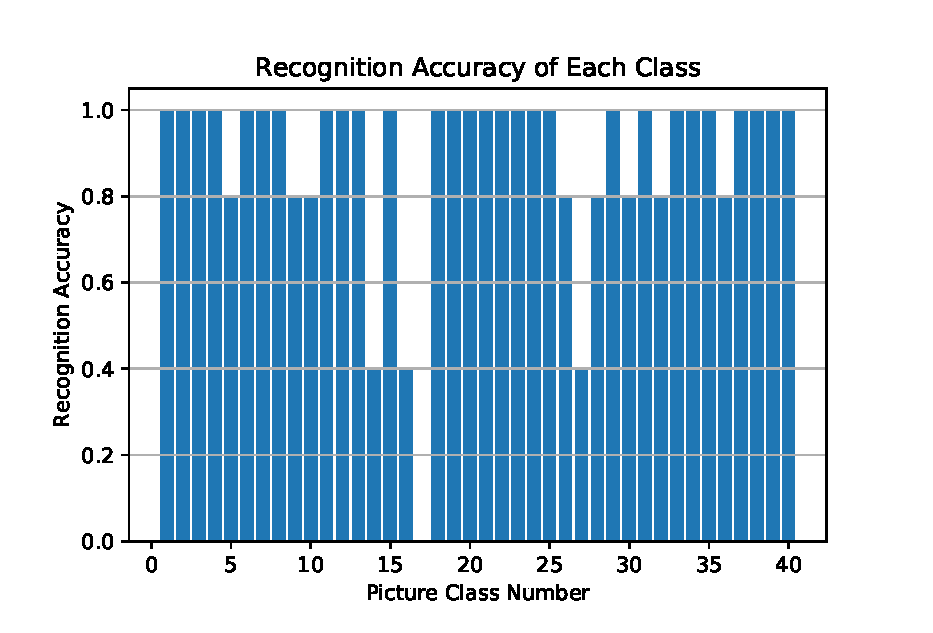
\includegraphics[scale = 0.6]{RA_Class.eps}
    \caption{各类别的识别精度}{滤波器:BOX;归一化方式:定值归一化;下采样倍数:20(即特征空间为56)}\label{fig-result_class_accuracy}
\end{figure}
其整体识别精度为92.5\%(保留一位小数),与原始文献中数据(93.5\%)相当,表\ref{tab-results_algorithms}中展示其他当时的领先算法使用同样的测试准则在AT\&T数据库中的表现。可见LRC在该数据库中的识别精度达到了接近同类算法的水平。\par
% \begin{table}[htbp]
%     \centering
%     \caption{不同算法在AT\&T数据库测试结果}\label{tab-results_algorithms}
%     \begin{tabular}{cc}
%         \toprule
%         \textbf{Approach} & \textbf{Recognition Rate} \\
%         \midrule
%         Fisherfaces & 94.50\% \\
%         \midrule
%         ICA & 85.00\% \\
%         \midrule
%         Kernel Eigenfaces & 94.00\% \\
%         \midrule
%         2DPCA & 96.00\% \\
%         \midrule
%         ERE & 97.00\% \\
%         \midrule
%         \textbf{LRC} & \textbf{93.50\%} \\
%         \bottomrule
%     \end{tabular}
% \end{table}
\begin{table}[htbp]
    \centering
    \caption{不同算法在AT\&T数据库测试结果}\label{tab-results_algorithms}
    \begin{tabular}{ccccccc}
        \toprule
        \textbf{Approach} & Fisherfaces & ICA & Kernel Eigenfaces & 2DPCA & ERE & \textbf{LRC} \\
        \midrule
        \textbf{Recognition Rate} & 94.50\% & 85.00\% & 94.00\% & 96.00\% & 97.00\% & \textbf{93.50\%} \\
        \bottomrule
    \end{tabular}
\end{table}
具体的实验数据可在附录中查看。

\section{总结与展望}\label{sec-4}
本文尝试理解并转述了文献\cite{5506092}中的有关内容,并在此基础上对文献中的用于面部识别的线性回归回归算法进行了重现并在AT\&T面部图像数据库上进行了测试,得到了与原始数据基本一致的实验结果。由于对统计学习的知识储备不足,以及时间问题,仅进行了一些小规模的实验探索了影响线性回归识别精度的一些细枝末节的内容,但最终还是对算法本身以及统计方法有了更深刻的认识。\par
最为直接的认识就是扩宽了眼界与想象力,此前无法想象线性回归这样的“经典”算法竟然能够用于人脸识别这样的“时髦”领域。虽然文章年代较老,但是还是令人印象深刻——经典和简单并不等效于低效,关键还是对问题和方法的认识是否透彻,会使用先进的方法是一层境界,但同时懂得何时不用先进方法可能是另一层境界。反而由于该算法简单快捷的特性使其能够适用于对运算性能要求较高的情景如视频图像识别等等。另外文中所述的模块化分割处理图像解决连续遮挡问题的方法也让人感到惊叹——当然也可能是因为自己在这方面知识储备不足而已。\par
此外,在实验中对一些图像处理的概念进行了学习。进一步地,编码过程中还一并学习了Python语言和LaTeX的有关知识,弥补了一直以来的知识空缺,受益匪浅。\par
回到算法层面:LRC算法本身可能还是具有一些不足。例如文中所述的适用于Yale B Datebase的subset 5即存在严重的照明变化的子集上的结果很差,可能该类问题无法直接用线性的方法去解决,非线性方法可能会是一个潜在的可能性,或者从图像处理的角度入手如何对图像进行处理令其适合线性回归的思路可能较为易于实现。另外该类方法应该较为依赖于训练数据的信息完整性,例如划分分块的方法如果在训练数据不是整个暴露出的面部的情况下结果一定很糟。另外文中所述的简单划分为等尺寸的方形区域用于处理连续遮挡的方法可能在遮挡形态较为复杂或范围较大的情况下并不适用。以上问题或许在其他人的工作中已经得以解决,虽然自己的研究方向并不在此,但出于兴趣,今后可考虑进一步阅读有关文献跟踪面部识别领域的新动向。
\appendix

\bibliography{reference} % 利用BibTeX 工具生成参考文献,不要带扩展名
\printindex % 利用makeindex 工具生成索引

\appendixpage
\section{代码}
\subsection{算法代码}
\begin{verbatim}
from __future__ import division  # 将整数/整数=整数的除法改为真正的除法
from PIL import Image  # 用于处理图像
import matplotlib.pyplot as plt  # 用于处理绘图
import numpy as np  # 用于操作矩阵
from utility import normalize_gray as normalize  # !在此选择归一化函数

# 全局参数
N = 40  # 图片总类数
Pn = 10  # 每类图片的总数
Pi = 5  # 每类图片训练集张数
Pj = Pn - Pi  # 每类图片的预测集张数

#! pillow中图像size表示是2-tuple: (width, height)
#! AT&T:(92, 112)
downsampling_sizes = [(round(92/40), round(112/40)), (round(92/35), round(112/35)), 
    (round(92/30), round(112/30)), (round(92/25), round(112/25)), (round(92/20), round(112/20)), 
    (round(92/14), round(112/14)), (round(92/10), round(112/10)), (round(92/5), round(112/5))]  # 不同轮次的重采样数据
sampling_type = Image.LANCZOS  # 重采样类型

overall_info = {}  # 不同轮次的结果存储

# 以不同重采样尺寸循环运行
for downsampling_size in downsampling_sizes:

    # 循环实验参数
    predictor = []  # 用于存储predictor的数组
    info = {'total_recognition_accuracy': 0.}  # 存储结果

    # 构建N个带有Pi个图片的predictor的数组
    i = 0
    while i < N:
        j = 0
        path1 = "orl_faces\\s"+str(i+1)+"\\"  # 第一层路径循环文件夹
        ims = []  # 初始化临时存储图片变量
        # 读取一组图片到list中
        while j < Pi:
            # 读取一张图片
            path = path1+str(j+1)+".pgm"  # 第二层路径循环图片文件
            im = Image.open(path)
            im.show()
            im = im.resize(downsampling_size, sampling_type)  # 重采样
            # 将该图片插入到该类数组中
            ims.append(list(im.getdata()))
            # 标准化
            normalize(ims[j])
            j += 1
        # 将ims转换为predictor并插入到数组中
        p = np.matrix(ims[0])  # 先插入头一个图片
        j = 1  # 此时j已经有一个
        # 将剩下的插入临时predictor
        while j < Pi:
            p = np.vstack((p, ims[j]))
            j += 1
        # 将predictor转置之后插入list
        predictor.append(p.T)
        i = i+1

    # 创建一个N*Pj大小的存储隶属类别的数组
    inner = []
    result = []
    # 创建一个待拷贝的长度为Pj的内链表
    for i in range(Pj):
        inner.append(0)
    # 以内链表进行拷贝创建隶属类别链表
    for i in range(N):
        result.append(inner.copy())

    # 将所有测试图片求取隶属类别
    i = 0
    while i < N:  # 外循环类别
        path1 = "orl_faces\\s"+str(i+1)+"\\"
        j = 0
        while j < Pj:  # 内层循环图片
            path = path1+str(j+Pi+1)+".pgm"  # 跳过前面Pi张训练图片
            test_im = Image.open(path)
            test_im = test_im.resize(downsampling_size, sampling_type)  # 重采样
            y = list(test_im.getdata())
            # 对y进行标准化
            normalize(y)
            # 转化为matrix并转置
            y = np.matrix(y).T
            dis = []
            for p in predictor:
                beta = np.dot(np.linalg.inv(np.dot(p.T, p)), np.dot(p.T, y))
                yhat = np.dot(p, beta)
                dis.append(np.sqrt(np.sum(np.square(y-yhat))))
            # 找到最小距离所在的索引位置,将之视作该图片从属的类别,记录之
            result[i][j] = dis.index(min(dis))+1
            j += 1
        i += 1
    # print(result)

    recognition_accuracy = []
    # 处理识别结果
    type_index = 1
    for type in result:
        recognition_accuracy.append(0.)
        for rec in type:
            if rec == type_index:
                recognition_accuracy[type_index-1] += 1
        recognition_accuracy[type_index -1] = recognition_accuracy[type_index-1]/Pj
        info['total_recognition_accuracy'] += recognition_accuracy[type_index-1]
        type_index += 1
    info['total_recognition_accuracy'] /= N  # 平均识别率
    # print("平均识别率:", recognition_accuracy)
    # print("总识别率:", info['total_recognition_accuracy'])
    run_key = int(downsampling_size[0]*downsampling_size[1])
    overall_info[run_key] = info['total_recognition_accuracy']

print(overall_info)
\end{verbatim}
\subsection{图表输出}
\begin{verbatim}
# 不同设置下算法表现折线图
r_box = ...
r_lanczos = ...
r_nearest = ...
r_box_minmax_norm = ...
r_lanczos_minmax_norm = ...
r_nearest_minmax_norm = ...

fig = plt.figure()

plt.plot(r_box.keys(),r_box.values(),'o-', label='BOX+256')
plt.plot(r_box_minmax_norm.keys(),r_box_minmax_norm.values(),'bo--', label='BOX+data')
plt.plot(r_lanczos.keys(),r_lanczos.values(),'*-', 
label = 'LANCZOS+256')
plt.plot(r_lanczos_minmax_norm.keys(),r_lanczos_minmax_norm.values(),'c*--', label = 'LANCZOS+data')
plt.plot(r_nearest.keys(),r_nearest.values(),'^-', 
label = 'NEAREST+256')
plt.plot(r_nearest_minmax_norm.keys(),r_nearest_minmax_norm.values(),'g^--', label = 'NEAREST+data')

plt.xlabel('Feature Dimension')
plt.ylabel('Recognition Accuracy')
plt.title('Recognition Accuracy with Respect to Feature Dimension')
plt.axis([0,400,0,1])

plt.legend()
plt.grid()
plt.savefig("RA_Method.pdf",format = "pdf")
plt.show()

# 使用表现最好的设置选项输出的每一组结果)
# 原始结果
i_result = ...
# 求出每组的成功率
i_recognition_accuracy = []
i_type_index = 1
for type in i_result:
    i_recognition_accuracy.append(0.)
    for i_rec in type:
        if i_rec == i_type_index:
            i_recognition_accuracy[i_type_index-1] += 1
    i_recognition_accuracy[i_type_index -1] = i_recognition_accuracy[i_type_index-1]/Pj
    i_type_index += 1
print(i_recognition_accuracy)

xl = np.arange(1,N+1)

plt.bar(xl,i_recognition_accuracy)
plt.xlabel('Picture Class Number')
plt.ylabel('Recognition Accuracy')
plt.title("Recognition Accuracy of Each Class")
plt.grid(axis = 'y')
plt.savefig('RA_Class.eps',format = 'eps')
plt.show()
\end{verbatim}


\section{详细实验数据}
\begin{table}[htbp]
    \centering
    \caption{不同设置下的LRC识别精度差异——详细实验结果}\label{tab-detailed_results}
    \begin{tabular}{ccccccccc}
        \toprule
        & \multicolumn{8}{c}{\textbf{Feature dimension}} \\
        \cmidrule{2-9}
        & 6 & 9 & 12 & 16 & 30 & 56 & 99 & 396 \\
        \midrule
        NEAREST+data & 0.07 & 0.22 & 0.375 & 0.525 & 0.680 & 0.805 & 0.845 & 0.870 \\
        \midrule
        NEAREST+256 & 0.05 & 0.240 & 0.375 & 0.605 & 0.710 & 0.820 & 0.850 & 0.875 \\
        \midrule
        BOX+data & 0.085 & 0.580 & 0.750 & 0.830 & 0.885 & 0.915 & 0.915 & 0.910 \\
        \midrule
        BOX+256 & 0.160 & 0.710 & 0.790 & 0.845 & 0.890 & \textbf{0.925} & 0.920 & 0.905 \\
        \midrule
        LANCZOS+data & 0.065 & 0.585 & 0.770 & 0.835 & 0.894 & 0.905 & 0.910 & 0.900 \\
        \midrule
        LANCZOS+256 & 0.100 & 0.675 & 0.815 & 0.885 & 0.920 & 0.915 & 0.915 & 0.905 \\
        \bottomrule
    \end{tabular}
\end{table}

 % 附录 appendix.tex
\end{document}
